\documentclass[addpoints,12pt]{exam}

\usepackage{amsmath}
\usepackage{amsthm}
\usepackage{graphicx}
\usepackage{enumitem}
\usepackage{amssymb}
\usepackage{tikz}
\usepackage{multicol}
\usepackage{comment}
\usepackage[margin = 0.5 in]{geometry}

\printanswers %Remove to hide answers
\pagestyle{headandfoot} %Adds Headers and Footers
\runningheadrule
\firstpageheader{Math 125}{Exam 1 Practice}{\today}
\runningheader{Math 125}
{Exam 1, Page \thepage\ of \numpages}
{\today}
\firstpagefooter{}{\thepage}{}
\runningfooter{}{\thepage}{}

\newcommand{\tft}{
\begin{oneparcheckboxes}
\CorrectChoice True
\choice False
	\end{oneparcheckboxes}
}
\newcommand{\tff}{
\begin{oneparcheckboxes}
\choice True
\CorrectChoice False
	\end{oneparcheckboxes}
}

\checkboxchar{$\Box$}
\checkedchar{$\blacksquare$}


\begin{document}

%The box at the top, and the name
\begin{center}
\fbox{\fbox{\parbox{5.5in}{\centering
Answer the questions in the spaces provided on the
question sheets. If you run out of room for an answer,
continue on the back of the page.}}}
\end{center}
\vspace{0.1in}
\makebox[\textwidth]{Name:\enspace\hrulefill}
\vspace{0.2in}

%Question Formatting
%\qformat{\textbf{Question \thequestion}\quad (\thepoints)\hfill}
%Point Table
\newtheorem{theorem}{Theorem}

%\begin{center}
%\gradetable[h][questions]
%\end{center}

%Beginning Questions
\begin{questions}
	\question Answer each of the following. \begin{enumerate}[label=\alph*)]
	    \item Give an example of a finite set $A$ in set builder notation. 
			\item Write this same set $A$ in roster method. 
			\item Give the cardinality $n(A)$ of your finite set $A$. 
			\item Give an example of a proper subset of your set $A$ if it exists. If there does not exist a proper subset, state why. Be sure to use proper notation when naming your subset, either using roster or set builder notation. 
			\item Is the set $\emptyset$ a subset of your set $A$?
	\end{enumerate}

	\begin{solution}
	    \begin{enumerate}[label = \alph*)]
	        \item  $A:= \{x\mid \text{x is a town in south dakota starting with $Y$. }\}$
					\item $A = \{\text{Yankton, Yale}\}$
					\item $n(A)=2$
					\item $\{\text{Yankton}\} \subset A$ 
					\item Yes! This is true no matter what set you choose for $A$. 
	    \end{enumerate}
	\end{solution}

	\question Consider the following two sets 
	\[
	A=\{a,b,c,d,e,f\} \hspace{30pt} B = \{d,e,f,g,h\}
	\]
	Answer the following True or False questions. 
	\begin{enumerate}[label = \alph*)]
		\item \tff $A\subseteq B$
		\item \tft $A\cap B = \{d,e,f\}$
		\item \tff $A\cup B = \{a,b,c,g,h\}$
		\item \tff $\{a,b,c,d,e,f\}\subset A$
		\item \tft $\{a,b,c,d,e,f\} \subseteq A$ 
		\item \tft $(B\subseteq B) \text{ and } (A\subseteq A)$ 
		\item \tft $A\cap B \subseteq A\cup B$
		\item \tff $a\in A$ and $b\in B$ 
		\item \tft $a\in A$ or $b\in B$ 
	\end{enumerate}

	\newpage

\question
Shade in the indicated subset in each Venn Diagram. 


\begin{multicols}{2}

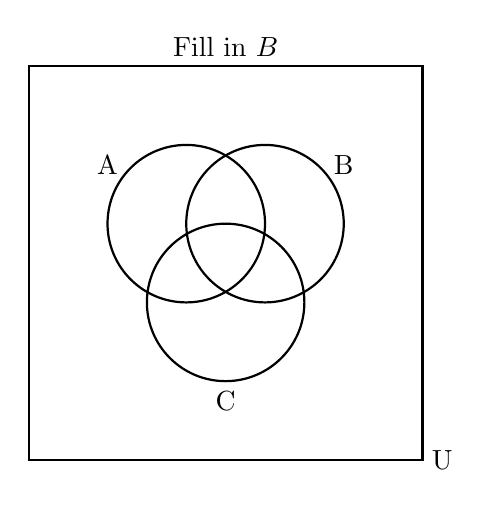
\begin{tikzpicture}
	\draw[black,thick] (0,0) rectangle (5,5) ;
\draw[black,thick] (2,3) circle (1);
\draw[black, thick] (3,3)circle (1);
\draw[black,thick] (2.5,2) circle (1);
\node (A) at (1,3.75){A};
\node (B) at (4,3.75){B};
\node (C) at (2.5,0.75) {C};
\node (U) at (5.25,0) {U};
\node (D) at (2.5,5.25) {Fill in $B$};
\end{tikzpicture}

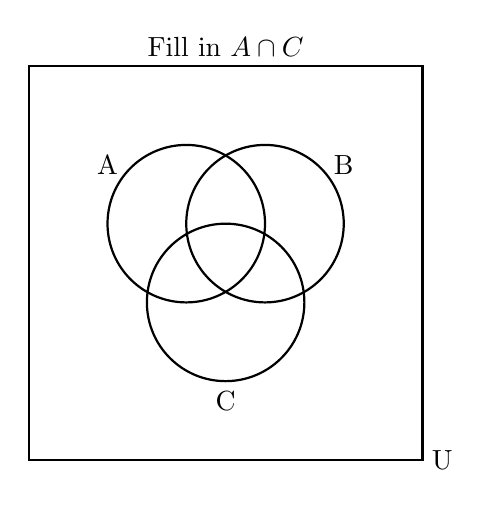
\begin{tikzpicture}
	\draw[black,thick] (0,0) rectangle (5,5) ;
\draw[black,thick] (2,3) circle (1);
\draw[black, thick] (3,3)circle (1);
\draw[black,thick] (2.5,2) circle (1);
\node (A) at (1,3.75){A};
\node (B) at (4,3.75){B};
\node (C) at (2.5,0.75) {C};
\node (U) at (5.25,0) {U};
\node (D) at (2.5,5.25) {Fill in $A\cap C$};

\end{tikzpicture}

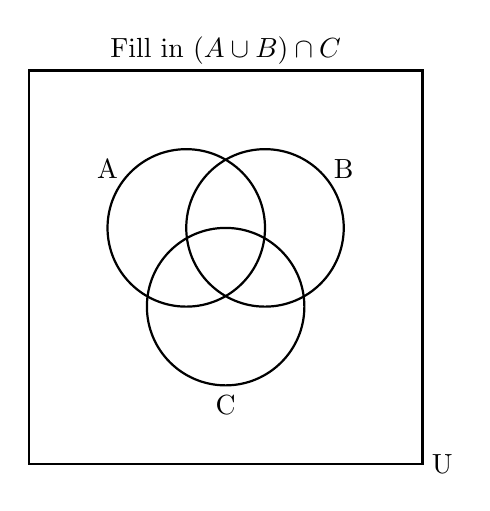
\begin{tikzpicture}
	\draw[black,thick] (0,0) rectangle (5,5) ;
\draw[black,thick] (2,3) circle (1);
\draw[black, thick] (3,3)circle (1);
\draw[black,thick] (2.5,2) circle (1);
\node (A) at (1,3.75){A};
\node (B) at (4,3.75){B};
\node (C) at (2.5,0.75) {C};
\node (U) at (5.25,0) {U};

\node (D) at (2.5,5.25) {Fill in $(A\cup B)\cap C$};

\end{tikzpicture}

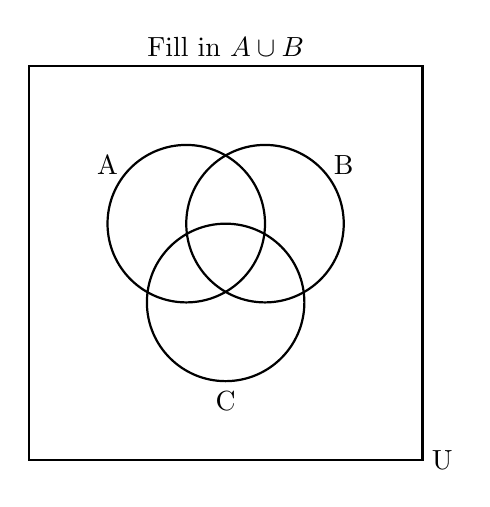
\begin{tikzpicture}
	\draw[black,thick] (0,0) rectangle (5,5) ;
\draw[black,thick] (2,3) circle (1);
\draw[black, thick] (3,3)circle (1);
\draw[black,thick] (2.5,2) circle (1);
\node (A) at (1,3.75){A};
\node (B) at (4,3.75){B};
\node (C) at (2.5,0.75) {C};
\node (U) at (5.25,0) {U};

\node (D) at (2.5,5.25) {Fill in $A\cup B$};

\end{tikzpicture}

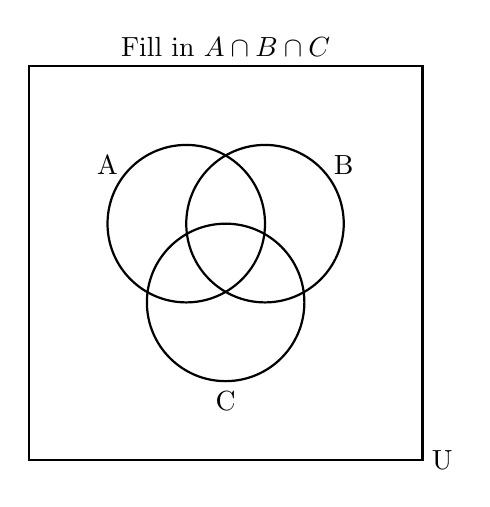
\begin{tikzpicture}
	\draw[black,thick] (0,0) rectangle (5,5) ;
\draw[black,thick] (2,3) circle (1);
\draw[black, thick] (3,3)circle (1);
\draw[black,thick] (2.5,2) circle (1);
\node (A) at (1,3.75){A};
\node (B) at (4,3.75){B};
\node (C) at (2.5,0.75) {C};
\node (U) at (5.25,0) {U};

\node (D) at (2.5,5.25) {Fill in $A\cap B\cap C$};

\end{tikzpicture}

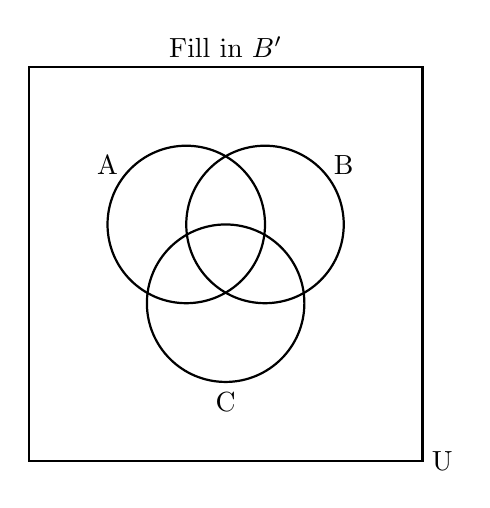
\begin{tikzpicture}
	\draw[black,thick] (0,0) rectangle (5,5) ;
\draw[black,thick] (2,3) circle (1);
\draw[black, thick] (3,3)circle (1);
\draw[black,thick] (2.5,2) circle (1);
\node (A) at (1,3.75){A};
\node (B) at (4,3.75){B};
\node (C) at (2.5,0.75) {C};
\node (U) at (5.25,0) {U};

\node (D) at (2.5,5.25) {Fill in $B'$};

\end{tikzpicture}

\end{multicols}

\newpage

\question Consider a poll where 44 people are asked if they eat Sauerkraut, Kimchi, and Miso. Let $A$ be the set of people that like Sauerkraut, $B$ be the set of people that like Kimchi, and $C$ be the set of people that like Miso. Consider the following pieces of information
\begin{itemize}
	\item We know 20 people like Sauerkraut. 
	\item We know 15 people like Kimchi. 
	\item We know 25 people like Miso.
	\item We know 7 people like Saurkraut and Kimchi
	\item We know 12 people like Sauerkraut and Miso. 
	\item We know 10 people like Kimchi and Miso. 
	\item We know 4 people like all 3. 
\end{itemize}

Fill in each region of the Venn Diagram with the number of people in each region. 

\begin{center}
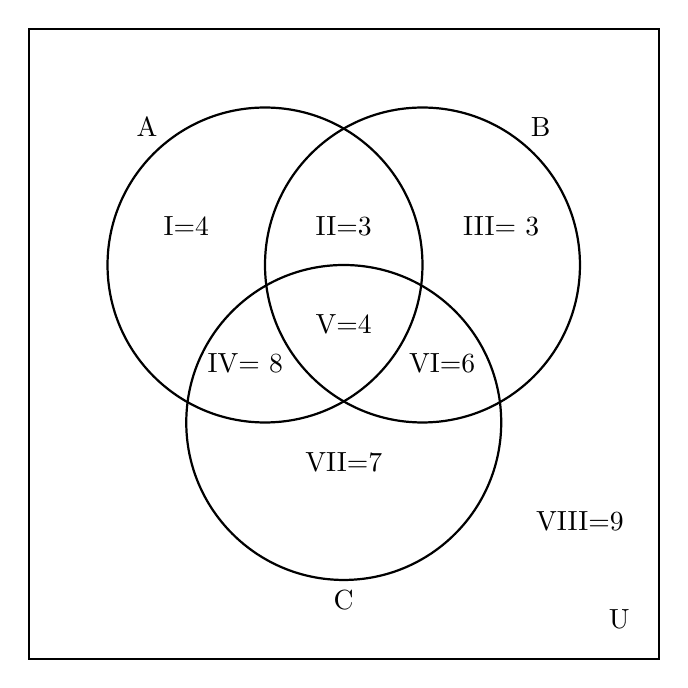
\begin{tikzpicture}
\draw[black,thick] (0,0) rectangle (8,8) ;
\draw[black,thick] (3,5) circle (2);
\draw[black, thick] (5,5) circle (2);
\draw[black,thick] (4,3) circle (2);
\node (A) at (1.5,6.75){A};
\node (B) at (6.5,6.75){B};
\node (C) at (4,0.75) {C};
\node (U) at (7.5,0.5) {U};
\node (3) at (2,5.5) {I=4};
\node (3) at (6,5.5) {III= 3};
\node (3) at (4,5.5) {II=3};
\node (3) at (2.75,3.75) {IV= 8};
\node (3) at (5.25,3.75) {VI=6};
\node (3) at (4,2.5) {VII=7};
\node (3) at (4,4.25) {V=4};
\node (3) at (7,1.75) {VIII=9};
\end{tikzpicture}
\end{center}

\begin{solution}
    See the filled in diagram above to get the final answers, but here is how we get each. 
		\begin{itemize}
		    \item Region V indicates all of the people that like Sauerkraut, Kimchi, and Miso. This is given to be 4 people. You must start with this region! 
				\item Next, Region II is all people that like Sauerkraut and Kimchi, but do not like Miso. The total of number of people that like Sauerkraut and Kimchi is 7 people. Therefore, we need to remove to people that also like Miso. Therefore, this region has $7-4=3$ poeple. 
				\item Next, Region  IV is the poeple like like Sauerkraut and Miso, but not Kimchi. In a similar thought process as the previous, we can see that this number of people is $12 - 4 = 8 $.  
				\item Next, region VI is the poeple like like Kimchi and Miso, but not Sauerkraut. In a similar thought process as the previous, we can see that this number of people is $10 - 4 = 6 $.  
				\item Region I is all people that only like Sauerkraut, and nothing else. Therefore, we can take the total number of people that like Sauerkraut, and remove the people from sections II, IV, and V that also like other things. Therefore, the total number of people in region I is  $20-4-9-3 = 4$. 
				\item Similar to the previous, the region III is all poeple that like Kimchi, but not the others. Therefore region II is $15-4-2-6= 3$. 
				\item Similar to the previous, the region VII is all people that like Miso, but not the others. Therefore region VII is $25-8-6-4 = 7$
				\item The last region VIII is obtained by removing all of the people that like at least $1$ of these foods from $44$ people total. Therefore, the number of people in region VIII is $44-7-8-6-4-3-3-4 = 9$

		\end{itemize}
\end{solution}
\newpage

\question Use the accompanying Venn diagram, which gives the cardinality of oeach region, to answer the questions below. 

\begin{enumerate}[label = \alph*)]
    \item How many elements below to set $B$? 
		\item How many elements belong to $A$ but not to $B$, that is, what is $n(A\cap B ')$?
		\item How many elements belong to set $A$ or set $B$,  that is, what is $n(A\cup B)$? 
		\item How many elements below to $B$ and $C$, that is, what is $n(B\cap C)$ ?
		\item How many elements belong in at least $1$ of the sets $A$, $B$ and $C$? that is, what is $n(A\cup B\cup C$)?

			Hint: $n(U) = 37$
\end{enumerate}

\begin{center}
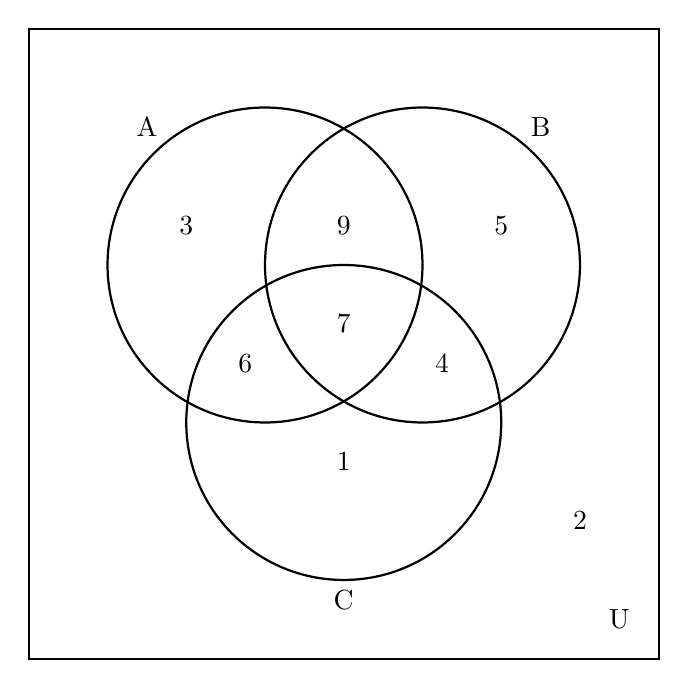
\begin{tikzpicture}
\draw[black,thick] (0,0) rectangle (8,8) ;
\draw[black,thick] (3,5) circle (2);
\draw[black, thick] (5,5) circle (2);
\draw[black,thick] (4,3) circle (2);
\node (A) at (1.5,6.75){A};
\node (B) at (6.5,6.75){B};
\node (C) at (4,0.75) {C};
\node (U) at (7.5,0.5) {U};
\node (3) at (2,5.5) {3};
\node (3) at (6,5.5) {5};
\node (3) at (4,5.5) {9};
\node (3) at (2.75,3.75) {6};
\node (3) at (5.25,3.75) {4};
\node (3) at (4,2.5) {1};
\node (3) at (4,4.25) {7};
\node (3) at (7,1.75) {2};
\end{tikzpicture}
\end{center}

\begin{solution}
    \begin{enumerate}[label = \alph*)]
			\item The set $B$ has $9+7+4+5 = 25$
			\item There are $3+6=9$ elements that are in $A$ but not in $B$. 
			\item There are $9+7+4+5+3+6 = 34$  elements in $A\cup B$. 
			\item There are $7+4$ elements of $B\cap C$. 
			\item There are $37-2=35$ elements of $A\cup B\cup C$. 
    \end{enumerate}
\end{solution}

\newpage
\question You take a poll of $100$ college students where classes at their college are held either Monday, Wednesday and Friday(MWF), or classes are help Tuesday and Thursday (TR). Assume every student is taking at least one class (they are students after all). If $65$ students report having classes $MWF$ and $55$ students report having classes on $TR$, how many people have class every day of the week? Hint: Use the inclusion-exclusion principle. 


\begin{theorem}[Inclusion-Exclusion Principle]
    Let $A$ and $B$ be finite sets. Then 
		\[
		n(A\cup B) = n(A)+n(B)-n(A\cap B)
		\]
\end{theorem}

\begin{solution}
	Let 
	\[
	A := \{p\mid p \text{ has class on MWF}\}
	\]
	\[
	B := \{p\mid p \text{ has class on TR}\}
	\]
	Then $n(A\cup B) = 100$ since this is just all the students. $A\cap B$ is the set we are interested in, which is students in class MWF and TR, which is all students. Therefore using the inclusion-exclusion principle
	\[
	n(A\cup B) = n(A)+n(B)-n(A\cap B)
	\]
	which if we substitute the given, we get 
	\[
	100 = 65+55 - n(A\cap B)
	\]
	Solving gives $n(A\cap B) = 65+55-100=20$. Therefore, there are $20$ students that have class every day of the week. 
    
\end{solution}\vfill


\question Let $A$, $B$ and $C$ be sets. Show explicitly that 
\[
n(A\cup B \cup C) = n(A)+n(B)+n(C) - n(A\cap B) - n(B\cap C) - n(A\cap C)+n(A\cap B \cap C)
\]
Verify this formula holds using the cardinalities given in Problem 4. 


\textbf{Hint:} $(A\cup B) \cap C = (A\cap B)\cup (B\cap C)$ and $(A\cap B) \cap (B\cap C) = A\cap B\cap C$. 

\textbf{Hint 2:} Use the inclusion-exclusion principle for two sets.  



 \textbf{Solution:}   First, use the inclusion exclusion principle on the set $A\cup B$ and the set $C$:
		\[
			\boxed{n((A\cup B)\cup C) = n(A\cup B)+n(C)-n((A\cup B)\cap C)}
		\]
		Then, using the fact that $(A\cup B)\cap C = (A\cap C)\cup (B\cap C)$
		we get :
		\[
			\boxed{n(A\cup B \cup C) = n(A\cup B)+n(C)-n((A\cap C)\cup (B\cap C))}
		\]
		Then, we need to use the inclusion exclusion prinicple on $n(A\cap B)$ :
		\[
			\boxed{n(A\cup B \cup C) = n(A)+n(B)-n(A\cap B)+n(C)-n((A\cap C)\cup (B\cap C))}
		\]
		Finally, we can use the inclusion exclusion principle on $(A\cap C)$ and $(B\cap C)$ :
\[
	\boxed{n(A\cup B \cup C) = n(A)+n(B)-n(A\cap B)+n(C)- \left(n(A\cap C)+n(B\cap C)-n((A\cap C)\cap (B\cap C))\right)}
\]
Distrubute the negative over the last 3 terms and use the fact that $(A\cap C)\cap (B\cap C)= (A\cap B\cap C)$ gives :
\[
	\boxed{n(A\cup B \cup C) = n(A)+n(B)+n(C)-n(A\cap B)-n(A\cap C)-n(B\cap C)+n(A\cap B\cap C)}
\]


\end{questions}


\end{document}
